\documentclass[a4paper]{article}

\usepackage[T1]{fontenc}
\usepackage{textcomp}
\usepackage[english]{babel}
\usepackage{hyperref}
\usepackage{amsmath, amssymb, amsthm}
\usepackage{geometry}
\usepackage{tikz-cd}

\usepackage{pgfplots}

% for including julia code
\usepackage[linenumbers]{jlcode}

% for vertically aligning images with text
\usepackage[export]{adjustbox}

% Remove indentation globally
\setlength{\parindent}{0pt}
% Have blank lines between paragraphs
\usepackage[parfill]{parskip}

\hypersetup{
    colorlinks = true, % links instead of boxes
    urlcolor   = cyan, % external hyperlinks
    linkcolor  = blue, % internal links
    citecolor  = cyan   % citations
}

\newcommand{\R}{\mathbb{R}}
\newcommand{\C}{\mathbb{C}}
\newcommand{\Q}{\mathbb{Q}}
\newcommand{\N}{\mathbb{N}}
\newcommand{\A}{\mathbb{A}}
\newcommand{\Z}{\mathbb{Z}}

% use bullets for items
\renewcommand{\labelitemii}{$\circ$}
\renewcommand{\Im}{\operatorname{Im}}

\newcommand\numberthis{\addtocounter{equation}{1}\tag{\theequation}}

\newtheorem{theorem}{Theorem}[section]
\newtheorem{lemma}{Lemma}[section]

\theoremstyle{definition}
\newtheorem{definition}{Definition}[section]

\theoremstyle{definition}
\newtheorem{example}{Example}[section]

\theoremstyle{remark}
\newtheorem*{remark}{Remark}

\theoremstyle{definition}
\newtheorem{exercise}{Esercizio}[section]
\newtheorem*{exercise*}{Esercizio}

\begin{document}
\begin{titlepage}
    \begin{sffamily}
        \begin{large}
            \begin{center}
                \vbox to 100pt{%
                        
\includegraphics[width=3cm]{cherubino}%
                        \vfil}
            \end{center}
            \begin{center}
                \begin{Large}
                    \uppercase{Universit\`a degli studi di Pisa}
                \end{Large}\\
                \rule{9cm}{.4pt}\\
                \smallskip
                Dipartimento di Matematica\\
                \medskip
                Corso di Laurea Triennale in
                Matematica\\
                \bigskip\vfill
                \begin{Large}
                    Laboratorio Computazionale
                \end{Large}\\
                \bigskip\bigskip\vfil
                \begin{Huge}
                    Parallel Homotopy Continuation in Julia
                \end{Huge}
                \bigskip\vfill
                \begin{tabular}{ll}
                    \textbf{Studente:}  & Francesco Minnocci \\
                    \textbf{Matricola:} & 600455
                \end{tabular}
            \end{center}
            \begin{center}
                \vfill
                \rule{9cm}{.4pt}\\
                \medskip
                \uppercase{Anno Accademico 2022 - 2023}\\
            \end{center}
        \end{large}
    \end{sffamily}
\end{titlepage}

\tableofcontents
\newpage

\section{Introduction}
Homotopy Continuation is a numerical method for solving systems of polynomial equations.
It is based on the idea of "deforming" a given system of equations into a simpler one whose
solutions are known, and then tracking the solutions of the original system as the deformation
is undone.

In this project, the method will be implemented in the Julia programming language, which is
particularly suited for scientific computing.
The primary source for this report is \cite{BertiniBook},
where the method is explained in much more detail.

\section{Homotopy Continuation}
We will only consider \textit{square} systems of polynomial equations, i.e. systems of $n$ polynomial equations in $n$ variables, although or over- or under-determined systems can
often be solved by reducing them to square systems, by respectively choosing a suitable square subsystem or squaring it by adding equations. Morever, we will restrict ourselves to
systems which have
isolated solutions, i.e. zero-dimensional varieties.

There are many ways to choose the "simpler" system, from now on called a \textit{start system}, but in general we can observe that, by Bezout's theorem, a system
$F=(f_1,\ldots,f_n)$ has at most $D:=d_1\ldots d_n$ solutions, where $d_i$ is the degre of $f_i(x_1,\ldots,x_n)$.

Therefore, we can build a start system of the same size and whose
polynomials have the same degrees, but whose solutions are easy to find, and thus can be used as starting points for the method.

For instance, the system $G=(g_1,\ldots g_n)$, where
$$ g_i(x_1,\ldots x_n)=x_i^{d_i}-1 ,$$
is such a system, since its zero locus is obtained by combining the $d_i$-th roots of unity in each variable, which are exactly $D$ points:
$$ \left\{\left(e^{\frac{k_1}{d_1}2\pi i},\ldots,e^{\frac{k_n}{d_n}2\pi i}\right),\text{ for }0\leq k_i\leq d_i-1\,\text{ and }i=1,\ldots,n\right\} .$$
\subsection{Choosing the homotopy}
The deformation between the original system and the start system is a \textit{homotopy}, for instance the convex combination of $F$ and $G$
\begin{equation}\label{eq:h1} H(x,t)=(1-t)F(x)+tG(x) ,\end{equation}
where $x:=(x_1,\ldots,x_n)$ and $t\in[0,1].$ This is such that the roots of $H(x,0)=G(x)$ are known, and the roots of $H(x,1)=F(x)$ are the solutions of the original system (the
reason why we place the start system at $t=0$ and the original system at $t=1$ is that we need higher numerical precision for the solutions of the original system, and there are more
floating point numbers near to $t=0$; see \cite{BertiniBook}, p. 33).
Therefore, we can implicitly
define a curve $z(t)$ in $\C^n$ by the equation \begin{equation}\label{eq:h2} H(z(t),t)=0,\end{equation} so that in order to approximate the roots of $F$ it is enough to numerically track $z(t)$.

To do so, we derive the expression \eqref{eq:h2} with respect to $t$, and get the \textit{Davidenko Differential Equation}
$$ \frac{\partial H}{\partial z}\frac{\mathrm{d} z}{\mathrm{d} t}+\frac{\partial H}{\partial t}=0 ,$$
where $\frac{\partial H}{\partial z}$ is the Jacobian matrix of $H$ with respect to $z$:
$$
    \frac{\partial H}{\partial z}=
    \begin{pmatrix}
        \frac{\partial H_1}{\partial z_1} & \cdots & \frac{\partial H_1}{\partial z_n} \\
        \vdots                            & \ddots & \vdots                            \\
        \frac{\partial H_n}{\partial z_1} & \cdots & \frac{\partial H_n}{\partial z_n}
    \end{pmatrix} .
$$
This can be rewritten as
\begin{equation}\label{eq:dav} \dot{z}=-\frac{\partial H}{\partial z}^{-1}\frac{\partial H}{\partial t} .\end{equation}
This is a system of $n$ first-order differential equations, which can be solved numerically for $z(t)$ as an initial value problem, which is called \textit{path tracking}.
\subsubsection{Gamma trick}
While \eqref{eq:h1} is a fine choice of a homotopy, it's not what it's called a \textit{good homotopy}: in order to ensure that the solution paths $z(t)$ for different roots
\begin{itemize}
    \item have no singularities, i.e. never cross each other for $t>0$ (at $t=0$ $F$ could have singular solutions), and
    \item don't go to infinity for $t\to 0$ (as $F$ could have a solution at infinity),
\end{itemize}
we can employ the \textit{Gamma trick}: this consists in modifying the linear homotopy
\eqref{eq:h1} by susbtituting the parameter $t\in[0,1]$ with a complex curve $q(t)$ connecting $0$ and $1$, such as
$$ q(t)=\frac{\gamma t}{\gamma t+(1-t)} ,$$
where $\gamma\in(0,1)$ is a random complex parameter.

This is a "probability one" procedure, i.e. for any particular system we can choose $\gamma$ outside of a finite amount of rays through
the origin to ensure that we get a good homotopy, basically because of the finiteness of the branch locus of the homotopy.
After substituting, we have
$$ H(x,t)=\frac{(1-t)}{\gamma t+(1-t)}F(x)+\frac{\gamma t}{\gamma t+(1-t)}G(x) ,$$
and by clearing denominators, we get our final choice of homotopy:
\begin{equation}\label{eq:h3} H(x,t)=(1-t)F(x)+\gamma tG(x) .\end{equation}
\subsection{Tracking down the roots}
We then need to track down individual roots, following the solution paths from
a root $z_0$ of the start system by solving the initial value problem associated to the Davidenko differential equation \eqref{eq:dav} with starting value $z_0$ and
$t$ ranging from $1$ to $0$.

This will be done numerically, by using a first-order predictor-corrector tracking method, whose typical iteration goes like this:
\begin{itemize}
    \item \textbf{Predictor:} we first apply Euler's method to get an approximation $\widetilde{z}_i$ of the next value of the solution path;
    \item \textbf{Corrector:} we then use Newton's method to correct $\widetilde{z}_i$ using equation \eqref{eq:h2}, so that it becomes a good approximation $z_i$ of the next value of the solution path.
\end{itemize}
In the following sections, we go into more detail on each of these steps.
\subsubsection{Predictor: Euler's method}
Recall that Euler's method consists in approximating the solution of the initial value problem associated to a system of first-order ordinary differential equations
\begin{equation*}
    \left\{
    \begin{aligned}
         & \dot{z}=f(z,t) \\
         & z(t_0)=z_0
    \end{aligned}
    \right.
\end{equation*}
by the sequence of points $(z_i)_{i\in\N}$ defined by the recurrence relation
$$ z_{i+1}=z_i+h\cdot f(z_i,t_i) ,$$
where $h$ is the step size.
In the case of the Davidenko equation \eqref{eq:dav}, we have
$$f(z,t)=-\left(\frac{\partial H}{\partial z}(z,t)\right)^{-1}\frac{\partial H}{\partial t}(z,t)$$ and $t_0=1$, since we are tracking from $1$ to $0$. For the same
reason, we set $$t_{i+1}=t_i-h.$$
\subsubsection{Corrector: Newton's method}
Since we want to solve $$H(z,t)=0,$$ we can use Newton's method to improve the approximation $\widetilde{z_i}$ obtained by Euler's method.
This is done by moving towards the root of the tangent line of $H$ at the current approximation, or in other words through the iteration
$$ z_{i+1}=z_i-\left(\frac{\partial H}{\partial z}(z_i,t_{i+1})\right)^{-1}H(z_i,t_{i+1}) ,$$
where this time $z_0=\widetilde{z}_i$, with $\widetilde{z}_i$ and $t_{i+1}$ obtained from the $i$-th Euler step.

Usually, only a few steps of Newton's method are needed; we chose a fixed number of 5 iterations.
At which point, we use the final value of the Newton iteration as the starting value for the next Euler step.
\subsubsection{Adaptive step size}
In order to improve the efficiency of the method, we will use an adaptive step size, which is based on the norm of the residual of Newton's iteration.
If the desired accuracy is not reached (say, when the norm of $H(z_i,t_i)$ is bigger than $10^{-8}$),
then we halve the step size; if instead we have 5 "successful" iterations in a row, we double the step size.

\section{Testing the method}
To test the method's scalability, we first launched it on a single-threaded machine, then one a multi-threaded one, and finally parallelized it on a Cluster.

The latter was done by using the Julia package \textit{Distributed.jl} to parallelize the tracking of the roots on separate nodes, and the \texttt{SlurmClusterManager} package, which allows
to run Julia code using the \texttt{Slurm} workload manager.

In order to scale the method to larger systems, we also implemented a random polynomial generator which can be found in \hyperref[sec:random]{random-poly.jl}; this was used to
evaluate the performance of the parallel implementation, by generating square systems of polynomials with normally distributed coefficients, each
polynomial having total degree less or equal to a fixed maximum degree.

The single-threaded machine and multi-threaded tests (which used the \texttt{@threads}
macro from the \textit{Threads.jl} package on the root tracking \texttt{for} loop in the file \hyperref[sec:listing]{solve.jl}) were run in order to visualize the real solutions of
small (2x2) systems: here, multi-threaded runs didn't improve the
performance on these smaller systems, as the overhead of multi-threading was too big compared to the actual computation time.

However, when testing a parallel implementation on larger randomly generated systems we observed an improvement in execution times on larger systems compared to the single-node
runs, as we show in the \hyperref[sec:parallel]{Results} section.

The Julia implementation for the tests described above can be found in Appendix \hyperref[sec:listing]{B}, while
the hardware specifications are listed in Appendix \hyperref[sec:hw]{A}.

\section{Possible Improvements}

\subsection{Homogenized Coordinates}

Since our start systems have the maximum number of solutions for its degree, some of them might converge to a point at infinity of our original system. In our current
implementation, we waste time by tracking them until reaching the maximum number of iterations.

To better treat such cases, we could view the system inside an affine patch of the projective plane, and using homogenized coordinates detect when a solution is going to infinity. This would involve homogenizing both systems and modifying the path-tracking algorithm for the detection of a point going to infinity.

\subsection{Predictor-Corrector}

Our (un)specific choice of predictor could be unsuitable for badly-conditioned systems; other software implementations of the homotopy continuation method use more accurate and numerically stable predictors, such as Runge-Kutta methods
\cite{HomotopyContinuation.jl}.

\section{Appendix A: Results}

\subsection{Single- and Multi-threaded}

Below are the plots of four different 2x2 systems for the single- (laptop) and multi- (desktop) threaded runs, with the real solutions being shown in
\textcolor{red}{red}:

\newgeometry{left=.3cm,top=0.1cm}
\begin{figure}[htb]
    \begin{tabular}{c c c}
        Single-threaded                                                          &   & Multithreaded \\
        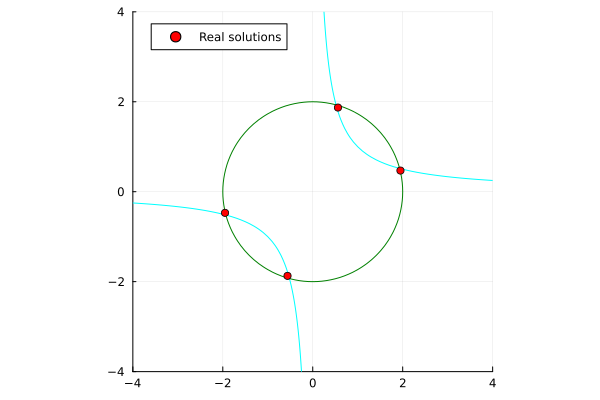
\includegraphics[width=0.45\textwidth,valign=c]{../plots/solutions1.png} &
        $\left\{\begin{aligned}
                         & x^3 + 5x^2 - y - 1 \\
                         & 2x^2 - y - 1       \\
                    \end{aligned}\right.$                                                 &
        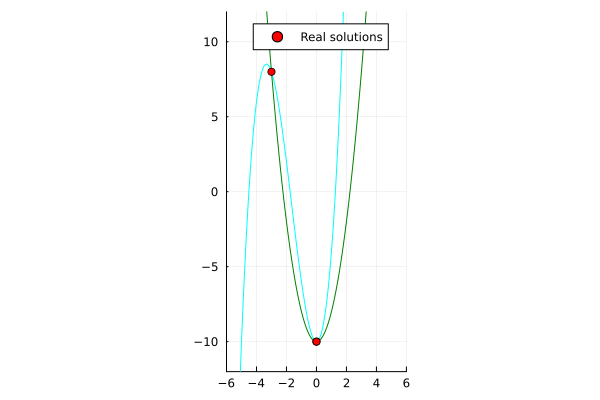
\includegraphics[width=0.45\textwidth,valign=c]{../plots/solutions1_6.png}                   \\
        \vspace{0.5cm}                                                                               \\
        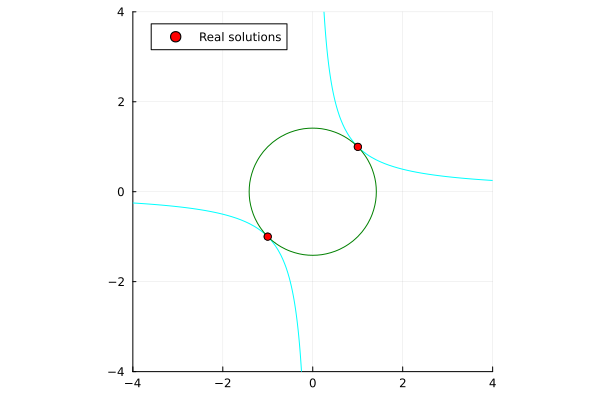
\includegraphics[width=0.45\textwidth,valign=c]{../plots/solutions2.png} &
        $\left\{\begin{aligned}
                         & x^2 + 2y \\
                         & y - 3x^3 \\
                    \end{aligned}\right.$                                                  &
        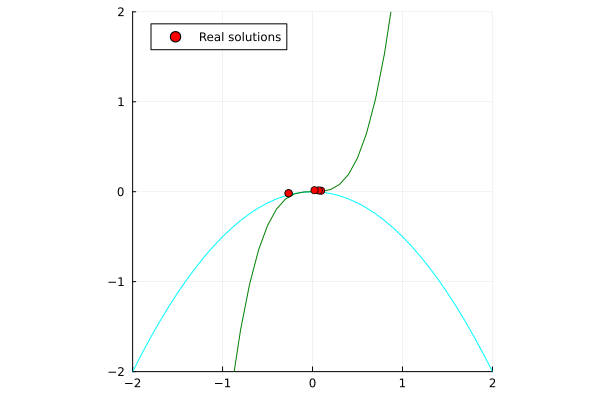
\includegraphics[width=0.45\textwidth,valign=c]{../plots/solutions2_6.png}                   \\
        \vspace{0.5cm}                                                                               \\
        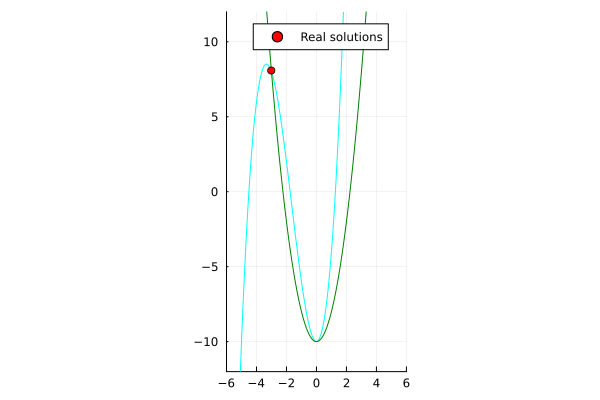
\includegraphics[width=0.45\textwidth,valign=c]{../plots/solutions3.png} &
        $\left\{\begin{aligned}
                         & x^2 + y^2 - 4 \\
                         & xy - 1        \\
                    \end{aligned}\right.$                                                  &
        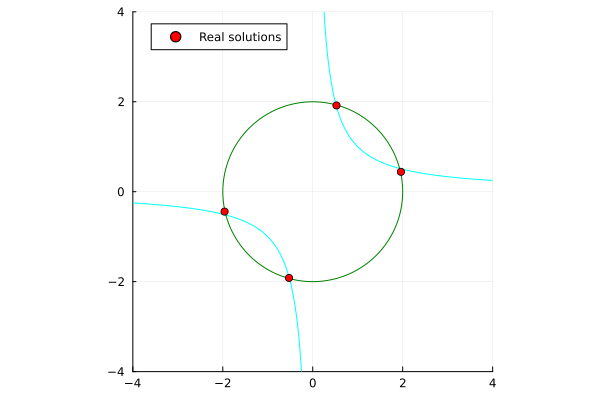
\includegraphics[width=0.45\textwidth,valign=c]{../plots/solutions3_6.png}                   \\
        \vspace{0.5cm}                                                                               \\
        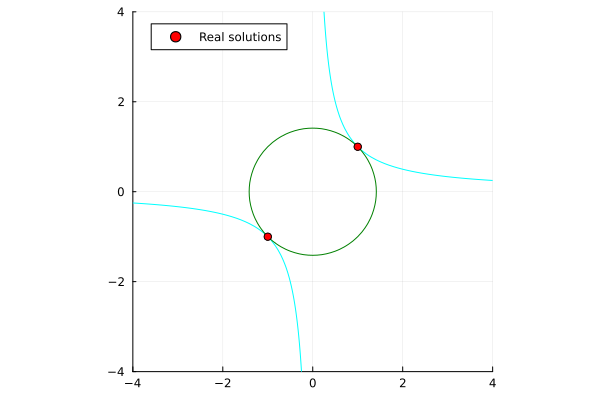
\includegraphics[width=0.45\textwidth,valign=c]{../plots/solutions4.png} &
        $\left\{\begin{aligned}
                         & x^2 + y^2 - 2 \\
                         & xy - 1        \\
                    \end{aligned}\right.$                                                  &
        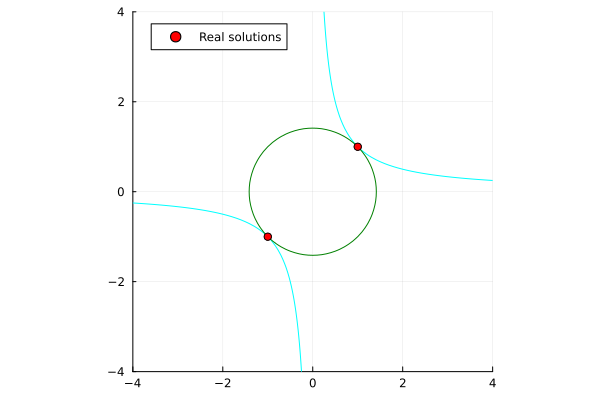
\includegraphics[width=0.45\textwidth,valign=c]{../plots/solutions4_6.png}                   \\
    \end{tabular}
\end{figure}

\restoregeometry

\subsection{Parallelization}\label{sec:parallel}

The following figure compares the execution times of the \texttt{solve} function in \hyperref[sec:listing]{solve.jl} on the cluster,
on a single node and on 20 nodes (using 1 or 2 threads per node).


\begin{figure}[htb]
    \centering
    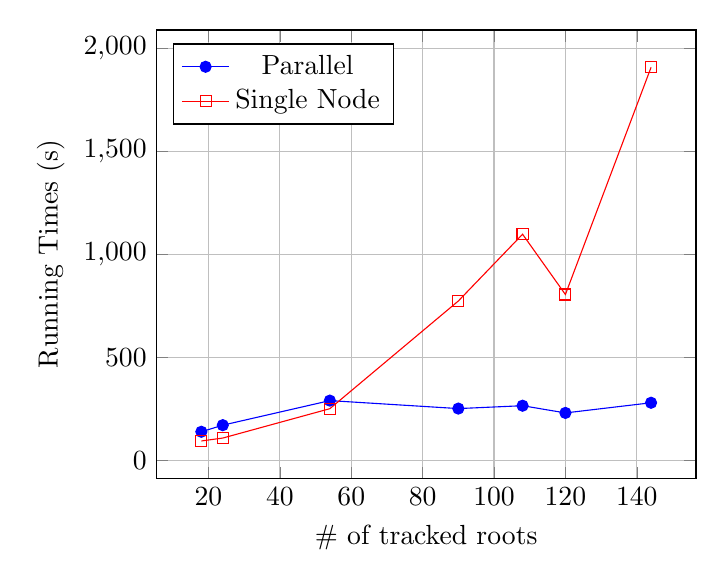
\begin{tikzpicture}
        \begin{axis}[
                xlabel={\# of tracked roots},
                ylabel={Running Times (s)},
                legend pos=north west,
                grid=major,
            ]

            \addplot[mark=*,blue] coordinates {
                    (18, 139.703750)
                    (24, 171.741583)
                    (54, 290.947457)
                    (90, 252.224948)
                    (108, 266.180392)
                    (120, 231.164993)
                    (144, 280.459045)
                };
            \addlegendentry{Parallel}

            \addplot[mark=square,red] coordinates {
                    (18, 95.067010)
                    (24, 109.203866)
                    (54, 251.746024)
                    (90, 774.436612)
                    (108, 1098.606851)
                    (120, 805.911525)
                    (144, 1908.437483)
                };
            \addlegendentry{Single Node}

        \end{axis}
    \end{tikzpicture}
    \caption{Performance comparison of parallel path tracking on a cluster.}
\end{figure}

As we can see from the plot, the parallel implementation appears to scale well with the number of tracked roots, and is faster than the single-node implementation for larger
systems.

\section{Appendix B: Implementation}
\subsection{Julia code}

The code is also available at the following GitHub repository:

\begin{center}
    \fbox{\url{https://github.com/bachoseven/homotopy-continuation}}
\end{center}

\label{sec:listing}\jlinputlisting[caption={solve.jl}]{../solve.jl}
\jlinputlisting[caption={start-system.jl}]{../start-system.jl}
\jlinputlisting[caption={homotopy.jl}]{../homotopy.jl}
\jlinputlisting[caption={homogenize.jl}]{../homogenize.jl}
\jlinputlisting[caption={euler-newton.jl}]{../euler-newton.jl}
\jlinputlisting[caption={adapt-step.jl}]{../adapt-step.jl}
\label{sec:random}\jlinputlisting[caption={random-poly.jl}]{../random-poly.jl}
\jlinputlisting[caption={plot.jl}]{../plot.jl}
\subsection{Hardware}\label{sec:hw}
For the single-threaded runs, the code was executed on a laptop with an Intel Core i7-3520M CPU @ 3.60GHz and 6 GB of RAM.

The multithreaded runs were tested on a desktop with an AMD FX-8350 CPU @ 4.00GHz with 4 cores and 8 threads, and 12 GB of RAM.

Finally, the parallel computations were run on a cluster with 20 nodes, each having a CPU @ 1.008GHz with 4 Performance cores, 2 efficiency cores and 4 GB of RAM.

\thebibliography{2}
\bibitem{BertiniBook} Bates, Daniel J. \textit{Numerically solving polynomial systems with Bertini}. SIAM, Society for Industrial Applied Mathematics, 2013.
\bibitem{Distributed.jl} https://docs.julialang.org/en/v1/stdlib/Distributed
\bibitem{HomotopyContinuation.jl} Breiding, P., Timme, S. (2018). HomotopyContinuation.jl: A Package for Homotopy Continuation in Julia. In: Davenport, J., Kauers, M., Labahn, G., Urban, J. (eds) Mathematical Software – ICMS 2018. Lecture Notes in Computer Science, vol 10931. Springer, Cham.
\end{document}
